\documentclass{template/newsreader}
\usepackage[utf8]{inputenc} % utf8 encoding
\usepackage{template/named}
\usepackage{fancyhdr}
\usepackage{fancyvrb}
\usepackage{multirow}
\setlength{\headheight}{15.2pt}

% TODOS
%
% @@ check optionality in all attributes


%%%%%%% Don't touch the following lines
%%%%%%% Taken from MEANING style
\newcommand {\deltitle}{\centering \LARGE {\textbf{\Title}}}
\DocTitle{\ShortTitle}
\DocNumber{{\WorkpackageNum}-{\DeliverableNum}}
\DocDate{\Date}
\DocVersion{\Version}
%%%%%%%
%%%%%%%


%% Warning: use 'pdflatex' command to compile this file.

%% Put here the title of the deliverable
\def\Title{NAF: NLP Annotation Format.}

%% The ``short'' title of the deliverable (in the case that \Title is too long)
%% This will be put in the header of the document. Let it be \Title in the case
%% is short enough
\def\ShortTitle{NAF}

%% Put here the authors
\def\Authors{Newsreader NAF team}

%% Put here the affiliation
\def\Affiliation{(1) EHU, (2) VUA, (3) FBK, (4) SynerScope}

%% The date
\def\Date{\today}

%% The Delivery Date
\def\DeliveryDate{--}

%% The workpackage number
\def\WorkpackageNum{WP2}

%% The workpackage responsible
\def\WPresponsible{Aitor Soroa}

%% The deliverable number (e.g. D2.1)
\def\DeliverableNum{NAF Deliverable}

%% The version of the document (e.g. DRAFT, FINA,...)
\def\Version{DRAFT}

%% Availability (Public / FP7 / IST / Project Internal)
\def\Availability{Public}

%% Type (report / prototype / software / ontology / wordnets /etc.)

\def\Type{Report}

%% Keywords
\def\Keywords{--}

%% Abstract
\def\Abstract{This document describes the specification of NAF.}

% \usepackage{listings,color}

% \definecolor{gray}{rgb}{0.4,0.4,0.4}
% \definecolor{darkblue}{rgb}{0.0,0.0,0.6}
% \definecolor{cyan}{rgb}{0.0,0.6,0.6}

% \lstset{
%   basicstyle=\ttfamily,
%   columns=fullflexible,
%   showstringspaces=false,
%   commentstyle=\color{gray}\upshape
% }

% \lstdefinelanguage{XML}
% {
%   basicstyle=\ttfamily\color{darkblue}\bfseries,
%   morestring=[b]",
%   morestring=[s]{>}{<},
%   morecomment=[s]{<?}{?>},
%   stringstyle=\color{black},
%   identifierstyle=\color{darkblue},
%   keywordstyle=\color{red},
%   morekeywords={xmlns,version,type}% list your attributes here
% }

\begin{document}

%\begin{document}
\begin{titlepage}
{
\center
%\framebox{
\begin{minipage}[t][3cm][c]{\textwidth}
\deltitle\\
\DeliverableNum\\
\small Version \Version
\end{minipage}
%}
}
\centering
\begin{minipage}[t][6cm][c]{\textwidth}
{\centering
% \begin{tabular}[h]{p{4cm}p{11cm}}
%  \textbf{Authors} &  \noindent   \begin{list}{}{\setlength{\itemsep}{0cm}} \item \Authors \end{list}  \\
 \begin{tabular}[h]{rp{13cm}}
   \textbf{Authors:} &  \Authors \\
   \textbf{Affiliation:} &  \Affiliation
 \end{tabular}
 \newline
}
\end{minipage}

%\vspace{.2cm}

{ \center
  \begin{minipage}{\textwidth}
    \centering
    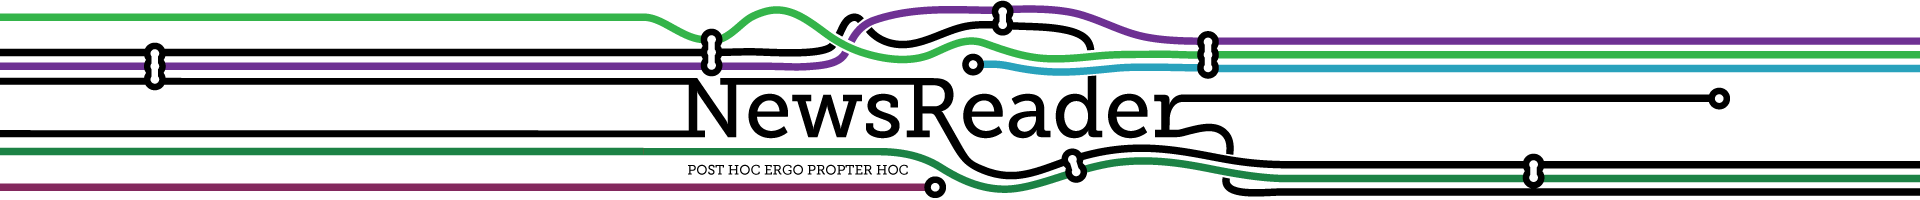
\includegraphics[width=\textwidth]{template/nwrLogo}
  \end{minipage}
}

\vspace{2cm}

{ \center
  \begin{minipage}{\textwidth}
    \centering
    
\includegraphics[width=.4\textwidth]{template/EULogos}
  \end{minipage}
}

%\vspace{2cm}

\centering
\textbf{
\begin{center}
  \small \sc Building structured event indexes of large volumes of financial and economic data for decision making\\
  ICT 316404
\end{center}
}

\end{titlepage}
\newpage

\newpage
%%
%% Informacio Segona Tapa
%%
 \begin{tabular}[h]{|p{8cm}|p{7cm}|} \hline
   \textbf{Grant Agreement No.} & 316404 \\ \hline
  \textbf{Project Acronym} & NEWSREADER\\ \hline
  \textbf{Project Full Title} & Building structured event indexes of large volumes of financial and economic data for decision making.\\ \hline
  \textbf{Funding Scheme} & FP7-ICT-2011-8\\ \hline
  \textbf{Project Website} & http://www.newsreader-project.eu/\\ \hline


  \textbf{Project Coordinator} & \begin{minipage}{7cm}
    \begin{tabular}{l}
      Prof. dr. Piek T.J.M. Vossen \\
      VU University Amsterdam \\
      Tel.  + 31 (0) 20 5986466 \\
      Fax. + 31 (0) 20 5986500 \\
      Email: piek.vossen@vu.nl      
    \end{tabular}
  \end{minipage} \\ \hline 
  \textbf{Document Number} &    \DeliverableNum \\ \hline
  \textbf{Status \& Version} & \Version \\ \hline
  \textbf{Contractual Date of Delivery} & \DeliveryDate \\ \hline
  \textbf{Actual Date of Delivery} & \today \\ \hline
  \textbf{Type} & \Type \\ \hline
  \textbf{Security (distribution level)} & \Availability \\ \hline
  \textbf{Number of Pages} & \pageref{LastPage} \\ \hline
  \textbf{WP Contributing to the Deliverable} & \WorkpackageNum \\ \hline
  \textbf{WP Responsible} & \WPresponsible \\ \hline
  \textbf{EC Project Officer} & Susan Fraser \\ \hline
  \multicolumn{2}{|p{15cm}|}{\textbf{Authors:}    \Authors } \\ \hline
  \multicolumn{2}{|p{15cm}|}{\textbf{Keywords:}  \Keywords} \\ \hline
  \multicolumn{2}{|p{15cm}|}{\textbf{Abstract:}  \Abstract} \\ \hline
  \end{tabular}
%%%%%%%%%%%%%%%%%%%%%%%%%%%%%%%%%%%%%%%%%%%%%%%%%%%%%%%%

%% Here starts the document


% \lstset{language=XML}

%% Revisions
\cleardoublepage
% \begin{nwrrevisions}
%  \nwrrevision{0.1}{Dec 2012}{An example document}{Author 1}{}
%  \nwrrevision{0.2}{Jan 2013}{Started with black document and created}{Author 2}{}
%  \nwrrevision{}{}{}{}{}
%  \nwrrevision{}{}{}{}{}
%  \nwrrevision{x.0}{date}{approval by project manager}{who}{-}
% \end{nwrrevisions}

% %% Excecutive Summary
% \cleardoublepage
% \section*{Executive Summary}

% executive summary text....


% %% TOC, tables
% \cleardoublepage
\tableofcontents
\cleardoublepage
\listoftables
\cleardoublepage

%%%%%%%%%%%%%%%%%%%%%%%%%%%%%%%%%%%%%%%
%%%%%%%%%%%%%%%%%%%%%%%%%%%%%%%%%%%%%%%
%%%%%%%%%%%%%%%%%%%%%%%%%%%%%%%%%%%%%%%
%%
%% Here starts the deliverable content.
%%
%%%%%%%%%%%%%%%%%%%%%%%%%%%%%%%%%%%%%%%
%%%%%%%%%%%%%%%%%%%%%%%%%%%%%%%%%%%%%%%
%%%%%%%%%%%%%%%%%%%%%%%%%%%%%%%%%%%%%%%

\section{Introduction}
\label{sec:introduction}

This document presents the first draft of NAF: NLP Annotation Format
to be used within the NewsReader project. This version of NAF evolves for
the format used in Kyoto, described in \cite{KAF}.


% @@
% [ASF: How about ``NLP Annotation Format'': since we're hoping NAF will be used beyond the project]

% @@TODO: add text. add references. add TAF, NIF, SEM\\

The following properties and desiderata are used as guidelines for defining NAF:

\begin{enumerate}
\item NAF should properly represent linguistic information focusing on two
  kind of linguistic processes (LPs):
  \begin{enumerate}
  \item within document processing: LPs whose granularity is the document
  \item cross document processing, for (event) coreference, etc.
  \end{enumerate}
  \item NAF should be simple
  \item NAF should work for existing NLP modules developed by the partners in NewsReader, i.e. it should be easy and little afford to adapt existing tools to use NAF.
  \item All elements in NAF will be identified with URIs (not document/XML-object internal ids)
  \item NAF should be flexible so that it can contain additional information and alternative representations:
  \begin{enumerate}
  \item It should be possible (and preferably easy) to integrate alternative modules (that may be developed by third parties) in the pipeline
  \item It should be possible to represent other RDF-based layers that link to the URIs used in the SEM annotation layer or to background knowledge
  \end{enumerate}
\end{enumerate}

The general approach for creating NAF will be to start with KAF, which already supports a number of desiderata mentioned above.
An overview of properties taken from KAF and proposed changes is given below:

\begin{enumerate}
  \item NAF will follow the stand-off/multi-layer architecture as also used in related formats such as KAF
  \item NAF will be presented in XML, using the KAF schema as a starting point
  \item The current ids in KAF will be converted to URIs
  \item Additional elements may be added, for instance, to allow for references to the SEM layer or background knowledge
  \item Elements may need to be reordered to turn KAF into a proper RDF graph
\end{enumerate}

% There have been numerous attempts to standardize some aspect of natural
% language processing. To date, the focus of standards (in various stages of
% development) includes morphosyntactic annotation (MAF) [3], syntactic
% annotation (SynAF) [4], and semantic annotation (e.g. SemAF [5]). The
% beforementioned standards concentrate on a specific stage of annotation. The
% two meta-models present different degrees of maturity; MAF has entered the
% last stages of the ISO process, whereas SynAF is at the level of Working
% Draft standard.

% A problem for these formats is that they are difficult to combine. For
% instance, we might want to do both syntactic annotation and semantic
% annotation, and integrate the results. The Linguistic Annotation Framework
% (LAF) [6] is an ISO standard proposal of a data model for linguistic
% annotation. It allows individual annotations within the annotation framework
% to refer to each other, so that the result is a combined analysis of the
% source text.

% Rather than a data model, our aim is a layered annotation format, where
% several processes can add information without losing anything which is
% produced by any previous process. NAF provides annotation layers for basic
% natural language processing and is open to extensions with other annotation
% layers needed by specific applications, which may be standardized later
% on. NAF is compatible with LAF but imposes a more specific standardization
% of the annotation format itself.

% NAF data format has been inspired by standard specifications available in
% the field of Language Resources. Basic motivations for that were to ensure
% intra- and inter-operability and portability. MAF and SynAF were
% investigated as far linguistic annotation for morpho-syntactic and syntactic
% information, respectively, is concerned.

% NAF can be seen as a three-layer format for text annotation: the first two
% layers, explicitly dedicated to representing morphosyntactic and syntactic
% information, are inspired by MAF and SynAF and are implemented "over" the
% semantic layer. For semantic annotation, the ISO community provides SemAF
% which is especially dedicated to the representation of events and time. We
% decided to boost semantic annotation and devised a dialect of the ISO
% standards, where semantic notation is tailored to the specific purposes of
% the project. NAF layers are to be seen as dialects of the ISO standards, yet
% maintaining (different degrees of) mappability to them. Therefore, NAF does
% not corrupt the compliance with ISO standards and their underlying
% philosophy; instead, it is in line with the strategy in ISO which provides
% high-level models (meta-models) able to be adapted, tailored and implemented
% according to specific needs.

NAF comprises several annotations over a text at different linguistic levels
(morphosyntactic, syntactic, semantic) and adopts a stand off strategy for
annotating the source text. The following overall rules are followed in all
layers:

\begin{itemize}
\item \texttt{<span>} elements are used for grouping linguistic elements.
\item Linguistic annotations of a particular level always span elements of previous levels.
\item Linguistic annotations of different levels are not mixed.
\end{itemize}


%%% Local Variables: 
%%% mode: latex
%%% TeX-master: "naf"
%%% End: 

\clearpage

\section{Root element}
\label{sec:root-element}

All NAF documents have a root element \texttt{<NAF>} which has the following
attributes:

\begin{itemize}
\item \texttt{xml:lang} (\textbf{required}): language identifier .
\item \texttt{version} (\textbf{required}): the version of NAF. For
  newsreader, we will use version \textbf{v1}
\end{itemize}

Example:
\begin{Verbatim}[fontsize=\small]
<NAF xml:lang="en" version="v3">
  <!--- ... --->
</NAF>
\end{Verbatim}

\section{NAF header}
\label{sec:naf-header}

NAF documents may have a header for describing information about the
document, such as its original name, URI or a list of the linguistic
processors which generated the NAF document. The NAF header is represented
within the \texttt{<nafHeader>} element, which is optional but highly
recommended. The header element has the following sub-elements:

\subsection{fileDesc element}
\label{sec:filedesc-element}

\texttt{<fileDesc>} is an empty element containing information about the
original document itself. It has the following attributes:
\begin{itemize}
\item \texttt{title} (optional): the title of the document.
\item \texttt{author} (optional): the author of the document.
\item \texttt{creationtime} (optional): a timestamp following the
  \emph{xs:dateTime}\footnote{See
      \texttt{http://www.w3.org/TR/xmlschema-2/\#isoformats}. In
    summary, the date is specified following the form
    ``YYYY-MM-DDThh:mm:ss'' (all fields required). To specify a time
    zone, you can either enter a dateTime in UTC time by adding a "Z"
    behind the time (``2002-05-30T09:00:00Z'') or you can specify an
    offset from the UTC time by adding a positive or negative time
    behind the time (``2002-05-30T09:00:00+06:00'').} format that
  specifies the time when the document was created.
\item \texttt{filename} (optional): the original file name.
\item \texttt{filetype} (optional): the original format (PDF, HTML, DOC, etc).
\item \texttt{pages} (optional): number of pages of the original document.
\end{itemize}

Example:

\begin{Verbatim}[fontsize=\small]
 <fileDesc creationtime="2014-01-01T00:00:00Z"
           title="The best residence in the world."
           author="casa400"
           filename="residence_hostal"
           filetype="PDF" pages="19"/>
\end{Verbatim}

% \subsection{dcDesc element}
% \label{sec:dcdesc-element}

% \texttt{<dcDesc>} is an element containing sub-elements that mimic those of
% the Dublin Core \footnote{dublincore.org/documents/dcmi-terms/}. The
% elements which describe various aspects of the original
% document. Specifically, we include those sub-elements:

% \begin{itemize}
% % \item \texttt{<title>}: A title for the document.
% \item \texttt{<creator>}: An entity primarily responsible for making the document.
% \item \texttt{<subject>}: The topic of the document.
% \item \texttt{<description>}: An account of the document.
% \item \texttt{<publisher>}: An entity responsible for making the document available.
% \item \texttt{<contributor>}: An entity responsible for making contributions to the document.
% \item \texttt{<date>}: A point or period of time associated with an event
%   in the lifecycle of the resource. The content of the element should be of
%   \emph{xs:dateTyme} type (see below).
% \item \texttt{<type>}: The nature or genre of the resource.
% \item \texttt{<format>}: The file format, physical medium, or dimensions of the resource.
% %\item \texttt{dcidentifier}: ---
% % \item \texttt{<source>}: A related resource from which the described resource is derived.
% % \item \texttt{<language>}: A language of the resource.
% % \item \texttt{<relation>}: A related resource.
% % \item \texttt{<coverage>}: The spatial or temporal topic of the resource,
% %   the spatial applicability of the resource, or the jurisdiction under which
% %   the resource is relevant.
% \item \texttt{<rights>}: Information about rights held in and over the resource.
% \end{itemize}

% Please note:
% \begin{itemize}
% \item The contents of each of those sub-elements are textual. Only the
%   \texttt{<date>} elements has a \emph{xs:datetime} type, so that date
%   expressions are normalized. In \ref{sec:ling-proc} section we describe the
%   format of this type.
% \item There can be any number of those subelements inside a
%   \texttt{<dcDesc>} element.
% \end{itemize}

% Example:

% \begin{Verbatim}[fontsize=\small]
% <dcDesc>
%   <description>An example document for explaining NAF.</description>
%   <creator>Aitor</creator>
%   <subject>Example</subject>
%   <subject>Small</subject>
% </dcDesc>
% \end{Verbatim}


\subsection{public element}
\label{sec:public-element}

\texttt{<public>} is an empty element which stores public information about
the document, such as its URI. It has the following attributes:
\begin{itemize}
\item \texttt{publicId} (optional): a public identifier (for instance, the
  number inserted by the capture server, or the MD5 hash number of the
  original document).
\item \texttt{uri} (optional): a public URI of the document.
\end{itemize}

Example:
\begin{Verbatim}[fontsize=\small]
  <public publicId="50ee45d106f9caf2d1cf38f29419efa8"
          uri="http://casa400.com/docs/residence.pdf"/>
\end{Verbatim}

\subsection{Linguistic Processors}
\label{sec:ling-proc}

The header also stores the information about which linguistic processors
produced the NAF document, described under \texttt{<linguisticProcessors>}
elements. There can be several \texttt{<linguisticProcessors>} elements, one
per NAF layer. NAF layers correspond to the top-level elements of the
documents, such as "text", "terms", "deps" etc.  Each
\texttt{<linguisticProcessors>} element contains one or several
\texttt{<lp>} elements, each one describing one specific linguistic
processor.\\

The \texttt{<lp>} element, if present, has the following attributes:
\begin{itemize}
\item \texttt{name} (\textbf{required}): the name of the processor
\item \texttt{version} (optional): processor's version
\item \texttt{timestamp} (optional): a timestamp, denoting the
  date/time at which the processor was launched. It follows the XML
  Schema \emph{xs:dateTime} format.
\item \texttt{beginTimestamp} (optional): a timestamp, denoting the
  date/time at which the processor started the process. It follows the XML Schema
  \emph{xs:dateTime} format.
\item \texttt{endTimestamp} (optional): a timestamp, denoting the date/time
  at which the processor ended the process. It follows the XML Schema
  \emph{xs:dateTime} format.
\end{itemize}

Example:

\begin{Verbatim}
<linguisticProcessors layer="text">
   <lp name="Freeling" version="2.1"
       timestamp="2012-06-25T10:05:00Z"
       beginTimestamp="2012-06-25T10:05:00Z"
       endTimestamp="2012-06-25T10:12:00Z"/>
 </linguisticProcessors>
 <linguisticProcessors layer="terms">
  <lp name="Freeling" version="2.1"
      timestamp="2012-06-25T10:10:19Z"
      beginTimestamp="2012-06-25T10:10:19Z"
      endTimestamp="2012-06-25T10:15:19Z"/>
  <lp name="ukb" version="0.1.2"
      timestamp="2012-06-25T16:10:19Z"
      beginTimestamp="2012-06-25T16:10:19Z"
      endTimestamp="2012-06-25T16:20:19Z"/>
</linguisticProcessors>
<linguisticProcessors layer="namedEntities">
  <lp name="Standfort_NE"
      version="0.1"
      timestamp="20090626_00:10:19Z"
      beginTimestamp="20090626_00:10:19Z"
      endTimestamp="20090626_00:14:19Z"/>
</linguisticProcessors>
\end{Verbatim}

Here is a full example of a NAF header:

\begin{Verbatim}
<nafHeader>
 <fileDesc creationtime="2014-01-01T00:00:00Z"
           title="The best residence in the world."
           author="casa400"
           filename="residence_hostal"
           filetype="PDF" pages="19"/>
  <public publicId="3_3012"
          uri="http://casa400.com/docs/residence.pdf" />
  <linguisticProcessors layer="text">
     <lp name="Freeling" version="2.1"
         timestamp="2012-06-25T10:05:00Z"
         beginTimestamp="2012-06-25T10:05:00Z"
         endTimestamp="2012-06-25T10:12:00Z"/>
   </linguisticProcessors>
   <linguisticProcessors layer="terms">
    <lp name="Freeling" version="2.1"
        timestamp="2012-06-25T10:10:19Z"
        beginTimestamp="2012-06-25T10:10:19Z"
        endTimestamp="2012-06-25T10:15:19Z"/>
    <lp name="ukb" version="0.1.2"
        timestamp="2012-06-25T16:10:19Z"
        beginTimestamp="2012-06-25T16:10:19Z"
        endTimestamp="2012-06-25T16:20:19Z"/>
  </linguisticProcessors>
  <linguisticProcessors layer="namedEntities">
    <lp name="Standfort_NE"
        version="0.1"
        timestamp="2009-06-26T00:10:19Z"
        beginTimestamp="2009-06-26T00:10:19Z"
        endTimestamp="2009-06-26T00:14:19Z"/>
  </linguisticProcessors>
</nafHeader>
\end{Verbatim}


%%% Local Variables: 
%%% mode: latex
%%% TeX-master: "naf"
%%% End: 

\clearpage

\section{Topics layer}
\label{sec:topics-layer}

This layer encodes the topics for the document. The topics correspond
to the whole document, and are usually assigned by authomatic methods,
such as text classification processors. The topics are annotated
within the \texttt{<topics>} element, and each topic is enclosed by a
\texttt{<topic>} element.

The \texttt{<topic>} element has the following attributes:
\begin{itemize}
\item \texttt{source} (optional): A reference to the entity
  responsible for creating the annotation.
\item \texttt{method} (optional): The name of the method used to
  create the annotation. This attribute is usually used in conjunction
  with the \texttt{source} attribute.
\item \texttt{confidence} (optional): this attribute is optional but
  its presence is highly recommended. It gives a value of
  ``confidence'' for the annotation. The confidence value can be in
  fact almost anything (similarity score, the value of the margin on a
  SVM based classification, etc), as long as it can be used to sort
  all annotations sharing the \texttt{source} and \texttt{method}
  attributes.
\item \texttt{uri} (optional): if the topic is a resource
  from an external reference, an URI to this resource. For instace, it
  could be a URI pointing to a Wikipedia category page, etc.
\end{itemize}

The content of the \texttt{<topic>} element is a string with the
topic.

Here is an example of topic annotation:

\begin{Verbatim}
<topics>
  <topic source="newsreader"
	 confidence="0.8"
	 method="textclassification-svm"
	 URI="http://en.wikipedia.org/wiki/Category:Tower_mills">
   Tower Mills</topic>
  <topic confidence="0.2"
	 source="newsreader"
	 method="textclassification-svm"
	 URI="http://en.wikipedia.org/wiki/Category:Windmills_in_Somerset">
   Windmills in Somerset</topic>
</topics>
\end{Verbatim}


%%% Local Variables: 
%%% mode: latex
%%% TeX-master: "naf"
%%% End: 

\clearpage

\section{Raw layer}
\label{sec:raw-layer}

NAF document can encode a ``raw'' layer with the actual document to be
processed. This layer is entirely optional, and is encoded as a
\texttt{CDATA} section.

Given this input document:
\begin{quote}
  John taught mathematics 20 minutes every Monday in New York.

  He liked it a lot!
\end{quote}

The NAF raw layer would look like:
\begin{verbatim}[fontsize=\small]
  <raw><![CDATA[John taught mathematics 20 minutes every Monday in New York.

He liked it a lot!]]>
  </raw>
\end{verbatim}


%%% Local Variables: 
%%% mode: latex
%%% TeX-master: "naf"
%%% End: 

\clearpage

\section{Word forms}
\label{sec:word-forms}

After tokenization step, all word forms are annotated within the
\texttt{<text>} element, and each form is enclosed by a \texttt{<wf>}
element.\\

The \texttt{<wf>} element has the following attributes:
\begin{itemize}
\item \texttt{id} (\textbf{required}): the unique id for the word form,
  starting with the prefix ``w''.
\item \texttt{offset} (\textbf{required}): The offset (in characters) of the
  original word form.
\item \texttt{lenght} (\textbf{required}): The lenght (in characters) of the
  original word form.
\item \texttt{sent} (\textbf{required}): sentence id of the token.
\item \texttt{para} (optional): paragraph id.
\item \texttt{page} (optional): page id.
\item \texttt{xpath} (optional): in case of source XML files, the xpath
  expression identifying the original word form.
\end{itemize}

NAF requires that input documents are encoded in UTF-8 and offsets are
described in characters. The purpose of the offset is to identify the source
string within the input document referred by the token, which is the string
starting at character \texttt{offset} and ending at \texttt{offset + length}
(exclusive).

The identifiers associated with sentences, paragraphs and pages
(\texttt{sent}, \texttt{para} and \texttt{page} attributes) have to be
numeric positive values in increasing order. The motivation is that the NAF
has to allow queries such as ``give me the words of the next (previous)
sentence'', which requires sentence identifiers to contain numbers.

The NAF tokenization looks like:
\begin{Verbatim}[fontsize=\small]
<text>
  <wf id="w1" offset="0" length="4" sent="1" para="1">John</wf>
  <wf id="w2" offset="5" length="6" sent="1" para="1">taught</wf>
  <wf id="w3" offset="12" length="11" sent="1" para="1">mathematics</wf>
  <wf id="w4" offset="24" length="2" sent="1" para="1">20</wf>
  <wf id="w5" offset="27" length="7" sent="1" para="1">minutes</wf>
  <wf id="w6" offset="35" length="5" sent="1" para="1">every</wf>
  <wf id="w7" offset="41" length="6" sent="1" para="1">Monday</wf>
  <wf id="w8" offset="48" length="2" sent="1" para="1">in</wf>
  <wf id="w9" offset="51" length="3" sent="1" para="1">New</wf>
  <wf id="w10" offset="55" length="3" sent="1" para="1">York</wf>
  <wf id="w11" offset="59" length="1" sent="1" para="1">.</wf>
  <wf id="w12" offset="62" length="2" sent="2" para="2">He</wf>
  <wf id="w13" offset="65" length="5" sent="2" para="2">liked</wf>
  <wf id="w14" offset="71" length="2" sent="2" para="2">it</wf>
  <wf id="w15" offset="74" length="1" sent="2" para="2">a</wf>
  <wf id="w16" offset="76" length="3" sent="2" para="2">lot</wf>
  <wf id="w17" offset="80" length="1" sent="2" para="2">!</wf>
</text>
\end{Verbatim}


%%% Local Variables: 
%%% mode: latex
%%% TeX-master: "naf"
%%% End: 

\clearpage

\section{Terms}
\label{sec:terms}

Terms are lexical units which refer to word forms (and groups multi word
forms). Terms are attached to several morphosyntactic information (such as
part of speech, lemma, etc), and may be linked to external resources like
WordNet senses, etc.\\

The \texttt{<term>} element has the following attributes:
\begin{itemize}
\item \texttt{id} (\textbf{required}): unique identifier starting with the
  prefix ``t''. If the term is a compound term (see Section
  \ref{sec:compound-terms}), the prefix is ``t.mw''.
\item \texttt{type} (optional): type of the term. Currently, 2 values are
  possible:
  \begin{itemize}
  \item \texttt{open}: open category term
  \item \texttt{close}: close category term
  \end{itemize}
\item \texttt{lemma} (optional): lemma of the term
\item \texttt{pos} (optional): part of speech. The first letter of the pos
  attribute must be one of the following:
  \begin{itemize}
  \item [N] common noun
  \item [R] proper noun
  \item [G] adjective
  \item [V] verb
  \item [P] preposition
  \item [A] adverb
  \item [C] conjunction
  \item [D] determiner
  \item [O] other
  \end{itemize}
\item \texttt{morphofeat} (optional): morphosyntactic feature encoded as a
  single attribute.
\item \texttt{head} (optional): if the term is a compound, the id of the
  head component (see Section \ref{sec:compound-terms}).
\item \texttt{case} (optional): declension case of the term.
\end{itemize}

The \texttt{<term>} element have the following sub-element:
\begin{itemize}
\item \texttt{span} (\textbf{obligatory)}: used to identify the tokens that
  the term spans. A single term may refer to one or more words, in case of
  multiword expressions. The \texttt{<span>} element has as many
  \texttt{<target>} sub-elements as spanned tokens (see example below).
\end{itemize}

Example of term level annotations:
\begin{Verbatim}[fontsize=\small]
<terms>
  <term id="t1" lemma="John" pos="R">
    <span>
      <target id="w1"/>
    </span>
  </term>
  <term id="t2" type="open" lemma="teach" pos="V">
    <span>
      <target id="w2"/>
    </span>
  </term>
  <term id="t3" lemma="mathematics" pos="N">
    <span>
      <target id="w3"/>
    </span>
  </term>
  <term id="t4" lemma="20" pos="N">
    <span>
      <target id="w4"/>
    </span>
  </term>
  <term id="t5" lemma="minute" pos="N">
    <span>
      <target id="w5"/>
    </span>
  </term>
  <term id="t5" lemma="every" pos="D">
    <span>
      <target id="w6"/>
    </span>
  </term>
  <term id="t6" lemma="Monday" pos="N">
    <span>
      <target id="w7"/>
    </span>
  </term>
  <term id="t7" lemma="in" pos="P">
    <span>
      <target id="w8"/>
    </span>
  </term>
  <term id="t.mw8" lemma="New_York" pos="R">
    <span>
      <target id="w9"/>
      <target id="w10"/>
    </span>
  </term>
</terms>
\end{Verbatim}


\subsection{Sentiment features}
\label{sec:sentiment-features}

The term layer represents sentiment information which is context-independent
and that can be found in a sentiment lexicon. It is related to concepts
expressed by words/ terms (e.g. ``beautiful'') or multi-word expressions
(e. g. ``out of order''). NAF provides possibilities to store sentiment
information at term level and at sense/synset level. In the latter case, the
sentiment information is included in the \texttt{<externalReference>}
section (Section \ref{sec:external-references}) and a word sense
disambiguation process may identify the correct sense along its sentiment
information. \\

%The extension contains the following information categories.

The \texttt{<sentiment>} element has the following attributes:
\begin{itemize}
\item \texttt{Resource} (\textbf{required}): identifier and reference to an external sentiment
  resource.
\item \texttt{Polarity} (\textbf{required}): Refers to the property of a
  word/sense to express positive, negative or no sentiment. These values are
  possible:
  \begin{itemize}
  \item positive
  \item negative
  \item neutral
  \item Or a numerical value.
  \end{itemize}
\item \texttt{Strength} (optional): refers to the strength of the polarity.
  \begin{itemize}
  \item weak
  \item average
  \item strong
  \item Or a numerical value
  \end{itemize}
\item \texttt{Subjectivity} (optional): refers to the property of a words to express an
  opinion (or not).
  \begin{itemize}
  \item subjective
  \item objective
  \item factual
  \item opinionated
  \end{itemize}
\item \texttt{Sentiment\_semantic\_type} (optional): refers to a
  sentiment-related semantic type. Possible values:
  \begin{itemize}
  \item Aesthetics\_evaluation
  \item Moral\_judgment
  \item Emotion
  \item etc.
  \end{itemize}
\item \texttt{Sentiment\_modifier} (optional): refers to words which modify
  the polarity of another word. Possible values:
  \begin{itemize}
  \item intensifier polarity shifter
  \item weakener polarity shifter
  \end{itemize}
\item \texttt{Sentiment\_marker} (optional): refers to words which
  themselves do not carry polarity, but are kind of vehicles of it. Possible
  values:
  \begin{itemize}
  \item Find, think, in my opinion, according to ...
  \end{itemize}
\item \texttt{Sentiment\_product\_feature} (optional): refers to a domain;
  mainly used in feature-based sentiment analysis. Values are related to
  specific domain. These are some possible values for for the tourist
  domain:
  \begin{itemize}
  \item staff, cleanliness, beds, bathroom, transportation, location, etc..
  \end{itemize}
\end{itemize}

Table \ref{tab:sent-attr-some} shows sentiment values for some words.

\begin{table}[t]
  \centering
  \ttfamily
  \small
  \begin{tabular}{|c|l|}
    \hline
    \textrm{Word} & \textrm{Sentiment attributes}\\
    \hline
    \multirow{6}{*}{\textrm{beatiful}} & polarity = "positive" \\
    & strength = "average" \\
    & subjectivity = "subjective"\\
    & sentiment\_semantic\_type = "aesthetics\_evaluation"\\
    & sentiment\_modifier = ""\\
    & sentiment\_product\_feature = "general"\\
    \hline
    \multirow{6}{*}{\textrm{valley}} & polarity = "negative"\\
    & strength = "average"\\
    & subjectivity = "factual"\\
    & sentiment\_semantic\_type = ""\\
    & sentiment\_modifier = ""\\
    & sentiment\_product\_feature = "beds"\\
    \hline
    \multirow{6}{*}{\textrm{very}} & polarity = ""\\
    & strength = ""\\
    & subjectivity = ""\\
    & sentiment\_semantic\_type = ""\\
    & sentiment\_modifier = "intensifier"\\
    & sentiment\_product\_feature = ""\\
    \hline
  \end{tabular}
  \caption{\textrm{Sentiment attributes.}}
  \label{tab:sent-attr-some}
\end{table}


Example:
\begin{Verbatim}[fontsize=\small]
<!-- term level sentiment annotation -->
<term id="t2" lemma="nice" pos="G">
  <sentiment resource="VUA_polarityLexicon_word" polarity="positive"
    strength="average" subjectivity="subjective"
    sentiment_semantic_type="behaviour/trait" />
  <span><target id="w2"/></span>
<!-- sense level sentiment annotation -->
</term>
<term id="t5" lemma="warm" pos="G">
  <sentiment/>
  <span><target id="w5"/></span>
  <externalReferences>
    <externalRef resource="WN-ENG" reference="c_1009" conf="0.38">
      <sentiment resource="VUA_polarityLexicon_synset" polarity="positive"
          strength="average" subjectivity="subjective"
         sentiment_semantic_type="behaviour/traitEvaluation"/>
    </externalRef>
    <externalRef resource="WN-ENG" reference="c_1008" conf="0.31">
      <sentiment resource="VUA_polarityLexicon_synset" polarity="positive"
         strength="average" subjectivity="objective"
         sentiment_semantic_type="temperature"/>
    </externalRef>
  </externalReferences>
</term>
\end{Verbatim}

\subsection{External References}
\label{sec:external-references}

The \texttt{<externalReferences>} element is used to associate terms to
external resources, such as elements of a Knowledge base, an ontology,
etc. It consists of several \texttt{<externalRef>} elements, one per
association. The \texttt{<externalRef>} elements may be nested, meaning that
each externalRef refines the relation expressed by the parent element.\\

The \texttt{<externalRef>} element has the following attributes:
\begin{itemize}
\item \texttt{resource} (\textbf{required}): indicates the identifier of the
  resource referred to.
\item \texttt{reference} (\textbf{required}): code of the referred
  element. If the element is a synset of some version of WordNet, it is
  recommended to follow the pattern:\\
  \begin{center}
    \texttt{[a-z]{3}-[0-9]{2}-[0-9]+-[nvars]}
  \end{center}
  which is a string composed by four fields separated by a dash. The four
  fields are the following:
  \begin{itemize}
  \item Language code (three characters, lowercase).
  \item WordNet version (two digits).
  \item Synset identifier composed by digits.
  \item POS character:
    \begin{itemize}
    \item [n] noun
    \item [v] verb
    \item [a] adjective
    \item [r] adverb
    \end{itemize}
  \end{itemize}
  examples of valid patterns are: ``eng-20-12345678-n'',
  ``spa-16-017403-v'', etc.
\item \texttt{reftype} (optional): indicates the kind of relation the
  externalRef is expressing.
\item \texttt{status} (optional): indicates the status of the relationship.
\item \texttt{source} (optional): the name of the process which created the
  external reference.
\item \texttt{confidence} (optional): a floating number between 0 and
  1. Indicates the confidence weight of the association.
\end{itemize}

Example of term level annotations:
\begin{Verbatim}[fontsize=\small]
<terms>
  <term id="t1" lemma="John" pos="R">
    <span>
      <target id="w1"/>
    </span>
  </term>
  <term id="t2" type="open" lemma="teach" pos="V">
    <span>
      <target id="w2"/>
    </span>
    <externalReferences>
      <externalRef resource="WN-1.7" reference="eng-17-00861095-v"
                   confidence="0.80">
        <externalRef resource="ontology" reference="Teach"
                     reftype="SubClassOf">
        </externalRef>
      </externalRef>
      <externalRef resource="WN-1.7" reference="eng-17-00859568-v"
                   confidence="0.20"/>
    </externalReferences>
  </term>
  <term id="t3" lemma="mathematics" pos="N">
    <span>
      <target id="w3"/>
    </span>
    <externalReferences>
      <externalRef resource="WN-1.7" reference="eng-17-04597590-n"
                   confidence="1.0"/>
    </externalReferences>
  </term>
  <term id="t4" lemma="20" pos="N">
    <span>
      <target id="w4"/>
    </span>
  </term>
  <term id="t5" lemma="minute" pos="N">
    <span>
      <target id="w5"/>
    </span>
  </term>
  <externalReferences>
    <externalRef resource="WN-1.7" reference="eng-17-12621100-n"
                 confidence="0.80"/>
    <externalRef resource="WN-1.7" reference="eng-17-12631889-n"
                 confidence="0.20"/>
  </externalReferences>
  <term id="t5" lemma="every" pos="D">
    <span>
      <target id="w6"/>
    </span>
  </term>
  <term id="t6" lemma="Monday" pos="N">
    <span>
      <target id="w7"/>
    </span>
    <externalReferences>
      <externalRef resource="WN-1.7" reference="eng-17-12557842-n"
                   confidence="1.0"/>
    </externalReferences>
  </term>
  <term id="t7" lemma="in" pos="P">
    <span>
      <target id="w8"/>
    </span>
  </term>
  <term id="mw8" lemma="New_York" pos="R">
    <span>
      <target id="w9"/>
      <target id="w10"/>
    </span>
  </term>
</terms>
\end{Verbatim}

\subsection{Compound terms}
\label{sec:compound-terms}

Compound terms can be represented in NAF by including \texttt{<component>}
elements within \texttt{<term>} elements. For example, the term
landbouwbeleid (English: agriculture policy) would look like this:

\begin{Verbatim}[fontsize=\small]
<term id="t.mw7" head="t.mw7.1" lemma="landbouwbeleid" pos="N" type="open">
  <span>
    <target id="w7"/>
    <target id="w8/>
  </span>
  <component id="t.mw7.1" lemma="landbouw" pos="N" type="open">
    <span>
     <target id="w7"/>
    </span>
    <externalReferences>...</externalReferences>
  </component>
  <component id="t.mw7.2" lemma="beleid" pos="N" type="open">
    <span>
     <target id="w8"/>
    </span>
    <externalReferences>...</externalReferences>
  </component>
  <externalReferences>...</externalReferences>
</term>
\end{Verbatim}

Note: the \texttt{id} attribute of compound terms start with the prefix ``t.mw''.\\

The \texttt{<component>} element has the same attributes and structure as
the \texttt{term} element, the only difference being that components can not
contain more \texttt{component} elements.

%%% Local Variables: 
%%% mode: latex
%%% TeX-master: "naf"
%%% End: 

\clearpage

\section{Dependency relations}
\label{sec:dependency-relations}

Dependencies represent dependency relations among terms. Each dependency is
represented by an empty \texttt{<dep>} element and span previous terms.\\

The \texttt{<dep>} element has the following attributes:
\begin{itemize}
\item \texttt{from} (\textbf{required}): term id of the source element
\item \texttt{to} (\textbf{required}): term id of the target element
\item \texttt{rfunc} (\textbf{required}): relational function. Among others,
  it can be one of:
  \begin{itemize}
  \item \texttt{mod}: indicates the word introducing the dependent in a
    head- modifier relation.  For instance:

    \begin{tabular}{ll}
      \texttt{mod(by,gift,Peter)} & the gift of a book by Peter\\
      \texttt{mod(of,examination,patient)} & the examination of the patient
    \end{tabular}

  \item \texttt{subj}: indicates the subject in the grammatical relation
    Subject-Predicate. For instance:

    \begin{tabular}{ll}
      \texttt{subj(arrive,John,\_)} & John arrived in Paris\\
      \texttt{subj(employ,Microsoft,\_)} &  Microsoft employed 10 C programmers\\
      \texttt{subj(employ,Paul,obj)} & Paul was employed by Microsoft
    \end{tabular}

  \item \texttt{csubj, xsubj, ncsubj}: The Grammatical Relations (RL) s
    csubj and xsubj may be used for clausal subjects, controlled from
    within, or without, respectively. ncsubj is a non-clausal subject. For
    instance:

    \begin{tabular}{ll}
      \texttt{xsubj(win,require,\_)} &  to win the America's Cup requires heaps of cash
    \end{tabular}

  \item \texttt{dobj}: Indicates the object in the grammatical relation
    between a predicate and its direct object. For instance:

    \begin{tabular}{ll}
      \texttt{dobj(read,book,\_)} & read books\\
    \end{tabular}

  \item \texttt{iobj}: The relation between a predicate and a non-clausal
    complement introduced by a preposition; type indicates the preposition
    introducing the dependent. For instance:

    \begin{tabular}{ll}
      \texttt{iobj(in,arrive,Spain)} &  arrive in Spain\\
      \texttt{iobj(into,put,box)} &  put the tools into the box\\
      \texttt{iobj(to,give,poor)} &  give to the poor
    \end{tabular}

  \item \texttt{obj2}: The relation between a predicate and the second
    non-clausal complement in ditransitive constructions. For instance:

    \begin{tabular}{ll}
      \texttt{obj2(head,dependent)} & \\
      \texttt{obj2(give,present)} &  give Mary a present\\
      \texttt{obj2(mail,contract)} & mail Paul the contract
    \end{tabular}
  \end{itemize}

\item \texttt{case} (optional): declension case
\end{itemize}

Example of dependency relation annotations:
\begin{verbatim}[fontsize=\small]
  <deps>
  <!-- subj(teach, John) -->
  <dep from="t1" to="t2" rfunc="subj" />
  <!-- dobj(teach, Mathematics) -->
  <dep from="t3" to="t2" rfunc="dobj" />
  <!-- iobj(teach, New_York) -->
  <dep from="t8" to="t2" rfunc="iobj" />
  </deps>
\end{verbatim}


%%% Local Variables: 
%%% mode: latex
%%% TeX-master: "naf"
%%% End: 

\clearpage
\section{Constituency parsing}
\label{sec:constituency-parsing}

This layer represent the output of constituency analysis parsers, i.e., full
syntactic tree of sentences. The top element of the layer is
\texttt{<constituency>}, and each sentence (parse tree) is represented by a
\texttt{<tree>} element. Inside each \texttt{<tree>}, there are three types
of elements:
\begin{itemize}
\item \texttt{<nt>} elements representing non-terminal nodes.
\item \texttt{<t>} elements representing terminal nodes.
\item \texttt{<edge>} elements representing in-tree edges.
\end{itemize}

The \texttt{<nt>} element represents the internal nodes of the parse
tree. It has the following attribute:
\begin{itemize}
\item \texttt{id} (\textbf{required}): unique identifier starting with the
  prefix ``nter'';
\item \texttt{label} (\textbf{required}): the category label of the node
  (for instance, 'S', 'NP', 'VP', etc).
\end{itemize}

The \texttt{<t>} element represents the leaf nodes of the parse tree. It has
the following attributes:
\begin{itemize}
\item \texttt{id} (\textbf{required}): unique identifier starting with the
  prefix ``ter'';
\end{itemize}

The \texttt{<t>} element contains a \texttt{<span>} element pointing to the
\emph{term} layer.  Each \texttt{<span>} contains one or more
\texttt{<target>} elements, with the following attributes:

\begin{itemize}
\item \texttt{id} (\textbf{required}): id of the target term.
\end{itemize}

The \texttt{<edge>} attribute links child nodes with its parent. It has the
following attribute:

\begin{itemize}
\item \texttt{id} (optional) unique identifier starting with the
  prefix ``tre'' (tree edge);
\item \texttt{from} (\textbf{required}): id of the child node. The child node can be a terminal
  or a non-terminal.
\item \texttt{to} (\textbf{required}): id of the parent node. The parent
  node is a non-terminal.
\item \texttt{head} (optional): a "yes" value indicates that the child node
  is the head constituent of the sub-tree pointed by the parent node.
\end{itemize}

Note that the order in which the \texttt{<edge>} elements appear in the XML
document is important. In particular, it has to maintain the relative order
among the sub-clauses of constituents. Therefore, in NAF the order of the
edges pointing to the same parent (having the same value for the \texttt{to}
attribute) has to be preserved.

Given the sentence:

\begin{quote}
  The dog ate the cat.  
\end{quote}

Its lispified parse tree is (heads are marked with an asterisk):
\begin{quote}
  (S (NP (DET The) *(NN dog)) *(VP *(V ate) (NP ((DET the) *(NN cat)))) (. .))
\end{quote}

The NAF representation would be as follows:

\begin{Verbatim}[fontsize=\small]
<constituency>
  <tree>
    <!-- Non-terminals -->
    <nt id="nter0"  label="ROOT"/>
    <nt id="nter1"  label="S"/>
    <nt id="nter2"  label="NP"/>
    <nt id="nter3"  label="VP"/>
    <nt id="nter4"  label="V"/>
    <nt id="nter5"  label="NP"/>
    <nt id="nter6"  label="DET"/>
    <nt id="nter7"  label="NN"/>
    <nt id="nter8"  label="DET"/>
    <nt id="nter9"  label="NN"/>
    <nt id="nter10" label="."/>
    <!-- Terminals -->
    <!-- The -->
    <t id="ter1"><span><target id="t1"/></span></t>
    <!-- dog -->
    <t id="ter2"><span><target id="t2"/></span></t>
    <!-- ate -->
    <t id="ter3"><span><target id="t3"/></span></t>
    <!-- the -->
    <t id="ter4"><span><target id="t4"/></span></t>
    <!-- cat -->
    <t id="ter5"><span><target id="t5"/></span></t>
    <!-- . -->
    <t id="ter6"><span><target id="t6"/></span></t>

    <!-- tree edges. Note: order is important! -->
    <edge id="tre1" from="nter1" to="nter0"/>             <!-- ROOT <- S -->
    <edge id="tre2" from="nter2" to="nter1"/>             <!-- S <- NP -->
    <edge id="tre3" from="nter6" to="nter2"/>             <!-- NP <- DET -->
    <edge id="tre4" from="ter1" to="nter6"/>              <!-- DET <- The -->
    <edge id="tre5" from="nter7" to="nter2" head="yes"/>  <!-- NP <- NN (head) -->
    <edge id="tre6" from="ter2" to="nter7"/>              <!-- NN <- dog -->
    <edge id="tre7" from="nter3" to="nter1" head="yes"/>  <!-- S  <- VP (head) -->
    <edge id="tre8" from="nter4" to="nter3" head="yes"/>  <!-- VP <- V (head) -->
    <edge id="tre9" from="ter3" to="nter4"/>              <!-- V  <- ate -->
    <edge id="tre10" from="nter5" to="nter3"/>            <!-- VP <- NP -->
    <edge id="tre11" from="nter8" to="nter5"/>            <!-- NP <- DET -->
    <edge id="tre12" from="ter4" to="nter8"/>             <!-- DET <- the -->
    <edge id="tre13" from="nter9" to="nter5" head="yes"/> <!-- NP <- NN (head) -->
    <edge id="tre14" from="ter5" to="nter5"/>             <!-- NN <- cat -->
    <edge id="tre15" from="ter6" to="nter10"/>            <!-- . <- . -->
    <edge id="tre16" from="nter10" to="nter1"/>           <!-- S <- . -->
  </tree>
</constituency>
\end{Verbatim}



%%% Local Variables: 
%%% mode: latex
%%% TeX-master: "naf"
%%% End: 

\clearpage

\section{Chunks}
\label{sec:chunks}

Chunks are noun or prepositional phrases, spanning terms.\\

The \texttt{<chunk>} element has the following attributes:
\begin{itemize}
\item \texttt{id} (\textbf{required}): unique identifier, starting with the prefix ``c''.
\item \texttt{head} (\textbf{required)}: the id of the chunk's head.
\item \texttt{phrase} (optional): type of the phrase.
\item \texttt{case} (optional): declension case.
\end{itemize}

Example of chunk annotations:
\begin{Verbatim}[fontsize=\small]
<chunks>
  <!-- John -->
  <chunk id="c1" head="t1" phrase="NP">
    <span>
      <target id="t1"/>
    </span>
  </chunk>
  <!-- taught -->
  <chunk id="c2" head="t2" phrase="V">
    <span>
      <target id="t2"/>
    </span>
  </chunk>
  <!-- Mathematics -->
  <chunk id="c3" head="t3" phrase="NP">
    <span>
      <target id="t3"/>
    </span>
  </chunk>
  <!-- 20 minutes -->
  <chunk id="c5" head="t5" phrase="NP">
    <span>
      <target id="t4"/>
      <target id="t5"/>
    </span>
  </chunk>
  <!-- every -->
  <chunk id="c6" head="t6" phrase="R">
    <span>
      <target id="t6"/>
    </span>
  </chunk>
  <!-- every Monday -->
  <chunk id="c7" head="t7" phrase="NP">
    <span>
      <target id="t6"/>
      <target id="t7"/>
    </span>
  </chunk>
  <!-- in New York -->
  <chunk id="c9" head="t9" phrase="PP">
    <span>
      <target id="t8"/>
      <target id="t9"/>
    </span>
  </chunk>
</chunks>
\end{Verbatim}


%%% Local Variables: 
%%% mode: latex
%%% TeX-master: "naf"
%%% End: 

\clearpage

\section{Named Entities}
\label{sec:named-entities}

Named entities are information units such as names, including person,
organization and location names, and numeric expressions including time,
date, money and percent expressions. NAF describes named entity mentions
present in text in a separate layer (\texttt{<entities>}), described in this
section. The \texttt{<entity>} element is used to represent a named entity
in the document. It may be used either for referencing single mentioned
entities or multi-mentioned entities: in the latter case, the element
contains clusters of term spans, which we call mentions, each mention
referencing the same entity. The text anchor is described by means of the
\texttt{<span>} elements, which always refer to term
elements. \texttt{<entity>} elements also annotates the type of the entity
mention. Besides, it can be linked to an external resource (such as
Wikipedia) using the \texttt{<externalRef>} element.

The \texttt{<entity>} element has the following attributes:
\begin{itemize}
\item \texttt{id} (\textbf{required}): unique id, starting with the prefix ``e''.
\item \texttt{type} (optional): named entity type. Some possible values:
  \begin{itemize}
  \item \texttt{Time}
  \item \texttt{Location}
  \item \texttt{Organization}
  \item \texttt{Person}
  \item \texttt{Money}
  \item \texttt{Percent}
  \item \texttt{Date}
  \item \texttt{Misc}
\end{itemize}
\item \texttt{source} (optional): the name of the process which created the
  entity.
\end{itemize}

The \texttt{<entity>} element has the following sub-elements:
\begin{itemize}
\item \texttt{<references>} (\textbf{required}): this element contains one or
  more \texttt{<span>} element, each one spaning terms.
\item \texttt{externalReferences} (optional): contains one or more
  \texttt{<externalRef>} element.
\end{itemize}

A \texttt{<span>} sub-element can be used to reference the different
occurrences of the same named entity in the document or mentions of it,
using \texttt{<target>} elements to refer to the terms it spans. If the
entity is composed by multiple words, multiple target elements are used.

The \texttt{<target>} element has the following attributes:
\begin{itemize}
\item \texttt{id} (\textbf{required}): id that refers to the target term.
\item \texttt{head} (optional): a "yes" value indicates that the term is the
  head of the mention.
\end{itemize}

The optional \texttt{<externalRef>} sub-element is used to associate terms
to external lexical or semantic resources. See Section
\ref{sec:external-references}.

Example of an entity mention:

\begin{Verbatim}[fontsize=\small]
<entities>
  <!-- John -->
  <entity id="e1" type="person">
    <references>
      <span>
        <target id="t1"/>
      </span>
    </references>
  </entity>
  <!-- New York -->
  <entity id="e2" type="location" source="spotlight-v07">
    <references>
      <span>
        <target id="t8"/>
      </span>
    </references>
    <externalReferences>
      <externalRef resource="Wikipedia"
                   reference="New_York"
                   confidence="0.85"/>
      <externalRef resource="Wikipedia"
                   reference="New_York,Lincolnshire"
                   confidence="0.15"/>
    </externalReferences>
  </entity>
  <!-- London -->
  <entity id="e3" type="location">
    <references>
      <!-- London -->
      <span>
        <target id="t12" head="yes"/>
      </span>
      <!-- The capital city of England -->
      <span>
        <target id="t1" />
        <target id="t2" />
        <target id="t3" head="yes"/> <!-- city is the head -->
        <target id="t4" />
        <target id="t5" />
      </span>
    </references>
    <externalReferences>
      <externalRef reference="ref01011020" 
                   resource="GeoNames"/>
      <externalRef reference="http://wwww.wikipedia.com/London" 
                   resource="Wikipedia"/>
    </externalReferences>
  </entity>
</entities>
\end{Verbatim}


%%% Local Variables: 
%%% mode: latex
%%% TeX-master: "naf"
%%% End: 

\clearpage

\section{Coreference}
\label{sec:coreference}

The coreference layer creates clusters of term spans (which we call
mentions) which share the same referent. For instance, ``London'' and ``the
capital city of England'' are two mentions referring to the same entity. It
is said that those mentions corefer.  A \texttt{<coref>} element represents
a mention cluster, and within \texttt{<coref>} each mention is represented
by a \texttt{<span>} element (which groups term mentions using
\texttt{<target>} elements). Additionally, one \texttt{<target>} element
within the \texttt{<span>} may have an attribute \texttt{head} with value
``yes'' to represent the fact that this particular term is the head of the
mention. For instance, the head of the mention ``the capital city of
England'' is ``city''.\\

The \texttt{<coref>} element has the following attribute:
\begin{itemize}
\item \texttt{id} (\textbf{required}): unique id, starting with the prefix ``co''.
\item \texttt{type} (optional): type of the coreference set. It describes
  whether the coreference cluster refers to an entity instance, and event,
  etc.
\end{itemize}

The \texttt{<coref>} element contains as many \texttt{<span>} elements as
elements in the coreference cluster. Each \texttt{<span>} contains one or
more \texttt{<target>} elements, with the following attributes:
\begin{itemize}
\item \texttt{id} (\textbf{required}): id that refers to the target term.
\item \texttt{head} (optional): a "yes" value indicates that the term is the
  head of the coreference cluster.
\end{itemize}

Example of a coreference cluster:

\begin{Verbatim}[fontsize=\small]
<coreferences>
  <coref id="co1" type="entity">
    <!-- London -->
    <span >
      <target id="t12" head="yes"/>
    </span>
    <!-- the capital city of England -->
    <span>
      <target id="t1"/>
      <target id="t2"/>
      <target id="t3" head ="yes"/> <!-- city is the head -->
      <target id="t4"/>
      <target id="t5"/>
    </span>
  </coref>
</coreferences>
\end{Verbatim}


%%% Local Variables: 
%%% mode: latex
%%% TeX-master: "naf"
%%% End: 

\clearpage

\section{Opinion layer}
\label{sec:opinion-layer}

The sentiment related information in NAF is represented at two levels: the
(already existing) term layer and a (new) opinion layer. The term layer
represents information copied from an external source like the sentiment
lexicon. Information can be stored at both word and sense-synset
level. Sentiment information in the term layer is the building block for the
sentiment analysis tool which then tries to generate information needed to
fill the slots (opinion holder, opinion target, opinion epression) of an
opinion triplet. These triplets are represented in the opinion
layer. Starting from these triplets, final sentiment analysis results can be
calculated.

Basic forms of sentiment analysis where polarity is aggregated at sentence
or document level may ignore the opinion layer triplets and make use of the
term level sentiment only. In these cases (for example, polarity
classification of product reviews) , opinion target (i. e. the product) and
opinion holder (i. e. the reviewer) are known on beforehand. However, when
more complex sentiment analysis is performed, the opinion triplets are
needed. An example of such an analysis, is product feature-based SA where
the target of the opinion is not just the product but some specific feature
of the product. Another example concerns the analysis of , for example, news
or blogs where different people (i. e. opinion holders) may have different
opinions about different targets. In those cases, aggregation of the
polarity values found in the text, is not enough.\\


The \texttt{<opinion>} element has one attribute:
\begin{itemize}
\item \texttt{id} (\textbf{required}): the unique identifier of the opinion,
  starting with the prefix ``o''.
\end{itemize}

The \texttt{<opinion>} element contains of the following subelements:
\begin{itemize}
\item \texttt{<opinion\_holder>}: the holder of the opinion, that is, the
  speaker or some actor in the text.
\item \texttt{<opinion\_target>} :  the target of the opinion (about what).
\item \texttt{<opinion\_expression>}: the opinion expression, which spans the
  terms comprising the opinion proper.
\end{itemize}
These three elements contain a \texttt{<span>} sub-element spanning terms.\\

The \texttt{<opinion\_holder>} element has the following attributes:
\begin{itemize}
\item \texttt{type} (optional): the type of the holder (for instance,
  ``Speaker/Writer'').
\end{itemize}

The \texttt{<opinion\_expression>} element has the following attributes:
\begin{itemize}
\item \texttt{polarity} (optional): refers to the positive or negative
  orientation of the expression.
\item \texttt{strength}: refers to the strength of the expression.
\item \texttt{subjectivity}: refers to whether an expression is subjective
  or not.
\item \texttt{sentiment\_semantic\_type}: refers to sentiment related
  semantic types like emotion, judgment, belief, speculation.
\item \texttt{sentiment\_product\_feature} : refers to specific features of
  entities, to be used in feature/aspect-based sentiment analysis.
\end{itemize}

% The fillers of the three elements (holder, target, type) can be found in one
% sentence or in different ones (cf. ex. 1). Moreover, one sentence can
% contain multiple opinion triplets (cf. ex. 2).


% Example

% (1)
% Vicky Masing,"http://twitter.com/VickyMasing/statuses/245094342799286273",2012-09-10T10:13:24Z,"english","Fountain of Bellagio Las Vegas. One has got to witness that magical show. Definitely beautiful, definitely mesmerizing."

% opinion expression: Definitely beautiful, definitely mesmerizing.
% polarity=positive, strength=strong, sentiment_semantic_type=evaluation,
% sentiment_product_feature=""
% opinion holder : Speaker/Writer
% opinion target : Fountain of Bellagio Las Vegas

% (2)
% We stayed at The Toren as a transit hotel for our trip from saudi arabia to USA, the hotel was just amazing in all aspects,
% the service was great, the people working their were really helpful and nice, the food at the breakfast was delicious and
% fresh and the location is great, very near to tram stops, the central station, Shopping...

% opinion expression:             really helpful and nice
% polarity:                               positive 
% strength:                               strong 
% sentiment_semantic_type:                evaluation
% sentiment_product_feature:      staff
% opinion holder :                        Speaker/Writer
% opinion target :                        people working there

% opinion expression:             delicious
% polarity:                               positive
%  strength:                      strong
%  sentiment_semantic_type:               evaluation
% sentiment_product_feature:      breakfast
% opinion holder :                        Speaker/Writer
% opinion target :                        the food at the breakfast

% (N.B. there are more opinion triplets in this fragment than the ones given here).


NAF Example:

\begin{Verbatim}[fontsize=\small]
<opinions>
  <!-- They had a nightmare with Hilton Hotel Paris. -->
  <opinion id="o1">
    <opinion_holder type="Speaker/Writer" >
      <span>
        <target id="t1"/>
      </span>
    </opinion_holder>
    <opinion_target>
      <span>
        <target id="t6"/>
        <target id="t7"/>
        <target id="t8"/>
      </span>
    </opinion_target>
    <opinion_expression polarity="negative" strength="strong" 
                        subjectivity="subjectivity"
                        sentiment_semantic_type="evaluation"
                        sentiment_product_feature="">
      <span>
        <target id="t3"/>
        <target id="t4"/>
      </span>
    </opinion_expression>
  </opinion>
</opinions>
\end{Verbatim}


%%% Local Variables: 
%%% mode: latex
%%% TeX-master: "naf"
%%% End: 

\clearpage

\section{Semantic Role Labeling}
\label{sec:semant-role-label}

Semantic Role Labeling (SRL) is a shallow semantic analysis which detects
semantic arguments associated with predicates. In NAF, the SRL information
is stored on a separate layer, whose top element is \texttt{<srl>}.

Each annotated predicate is represented by an \texttt{<predicate>}
element. The \texttt{<predicate>} element has the following attributes:
\begin{itemize}
\item \texttt{id} (\textbf{required}): the identifier of the predicate,
  starting with the prefix ``pr''.
\item \texttt{uri} (optional): An URI to an external resource representing the model of
  an event/predicate. For instance, it could be a reference to a frame in
  \emph{FrameNet} (@@rref), \texttt{PropBank} (@@rref), etc.
\item \texttt{confidence} (optional): a floating number between 0 and
  1. Indicates the confidence weight of the association.
\end{itemize}


Inside \texttt{<predicate>}, there are the following sub-elements:
\begin{itemize}
\item One \texttt{<externalReferences>} element, which links the predicate
  with one or more external resources.
\item One \texttt{<span>} element, spaning terms, and which point to the
  surface form of the predicate in the document.
\item One or more \texttt{<role>} elements which fill the arguments of the
  predicate.
\end{itemize}

As always in NAF, the \texttt{<span>} element contains one or more
\texttt{<target>} elements with the following attribute:

\begin{itemize}
\item \texttt{id} (\textbf{required}): id of the target term.
\end{itemize}

The \texttt{<role>} element represents filler of a particular argument of
the predicate. It has the following attributes:
\begin{itemize}
\item \texttt{id} (\textbf{required}): the id of the role, starting with
  prefix ``rl''.
\end{itemize}

Inside \texttt{<role>}, there are the following sub-elements:
\begin{itemize}
\item One \texttt{<externalReferences>} element, which links the predicate
  with one or more external resources.
\item One \texttt{<span>} element, spaning terms, and which point to the
  surface form of the predicate in the document.
\end{itemize}

Each \texttt{<span>} contains one or more \texttt{<target>}
elements, with the following attributes:

\begin{itemize}
\item \texttt{id} (\textbf{required}): id of the target term.
\end{itemize}

Given the following sentence:

\begin{quote}
  She was making apple jam for her friends and it was a surprise.
\end{quote}

The SRL layer would be encoded as follows:

\begin{verbatim}[fontsize=\small]
<srl>
  <predicate id="pr1" uri="http://framenet.net/Make" confidence=0.9>
    <!-- making -->
     <externalReferences>
        <externalRef reference="cognition" reftype="mcr:cognition" resource="2"/>
        <externalRef reference="cognition" reftype="mcr:cognition" resource="mc"/>
        <externalRef reference="eng-30-00690614-v" resource="wn:eng-30"/>
      </externalReferences>
    <span>
      <target id="t3"/>
    </span>
    <role id="rl1" semRole="Agent">
      <!-- She -->
      <externalReferences>
        <externalRef reference="participant" resource="1"/>
      </externalReferences>
      <span>
	<target id="t1"/>
      </span>
    </role>
    <role id="rl2" semRole="Theme">
      <!-- apple jam -->
      <span>
	<target id="t4"/>
	<target id="t5"/>
      </span>
    </role>
  </predicate>
</srl>
\end{verbatim}


%%% Local Variables: 
%%% mode: latex
%%% TeX-master: "naf"
%%% End: 

\clearpage

\section{Time expressions and events}
\label{sec:time-expr-events}

This section describes representing relations among events, events and time
expressions, or relations among time expressions. We first describe how to
represent events and time relations. Then, we describe how to represent
relations among them.

\subsection{Events}
\label{sec:events}

Within NAF, events are represented as coreference clusters in the
coreference layer \ref{sec:coreference}. Thus, the way to refer to those
events is to just span to a coreference element (c.f. Section
\ref{sec:coreference}). For instance, the following example:

\begin{Verbatim}
<coreferences>
  <coref id="coevent2" type="event">
    <span>
      <!--liked-->
      <target id="t13"/>
    </span>
  </coref>
  <coref id="coevent1" type="event">
    <span>
      <!--taught-->
      <target id="t2"/>
    </span>
  </coref>
</coreferences>
\end{Verbatim}

\noindent the coreference clusters \texttt{coevent2} and
\texttt{coevent1} (of type ``event'') represent two events.

\subsection{Time expressions}
\label{sec:time-expressions}

NAF follows TimeML schema for annotating time expressions under the
\texttt{timeExpressions} layer. Inside \texttt{timeExpressions} there are
many \texttt{<timex3>} elements, each one describing one time
expression. The \texttt{<timex3>} in NAF have the same semantics as
TimeML. The only difference is that TimeML inserts \texttt{<timex3>}
elements along with the running text in the document, wheras NAF uses a
stand-off approach. Please refer to TimeML specification document
\cite{isotimeml} for further information.

The \texttt{<timex3>} element has the following attributes:
\begin{itemize}
\item \texttt{id} (\textbf{required}): unique identifier starting with
  the prefix ``tmx'' (``tmx1'', ``tmx2'', etc.)

\item \texttt{type} (\textbf{required}): type of the timex3
  expression. Possible values:
  \begin{itemize}
  \item DATE
  \item TIME
  \item DURATION
  \item SET
  \end{itemize}

\item \texttt{beginPoint} (optional): id of a \texttt{timex3} element that
  represents the beginning point of a duration.
\item \texttt{endPoint} (optional): id of a \texttt{timex3} element that
  represents the end point of a duration.
\item \texttt{quant} (optional): used for specifying sets that denote
  quantified times. Generally a literal from the text that quelifies over
  the expression. Usual values are ``EVERY'', ``SOME'', etc.
\item \texttt{freq} (optional): Used for specifying sets that denote
  quantified times. It contains an integer value and a time granularity to
  represent any frequency contained in the set. Usual values are ``2X''
  (twice-a-month), ``3D'' (three-days), etc.

\item \texttt{functionInDocument} (default value: ``NONE''): indicates the
  function of the timex3 providing an anchor to other temporal expressions
  in the document. One of this values:

  \begin{tabular}{|c|p{9cm}|}
    \hline
    Value & Description \\
    \hline
    CREATION\_TIME     & date and time the identified resource where first created.\\
    EXPIRATION\_TIME   & date and time when the right to publish material expires.\\
    MODIFICATION\_TIME & date and time the resource was last modified.\\
    PUBLICATION\_TIME  & date and time when the resource is released to the public.\\
    RELEASE\_TIME      & date and time when the resource may be distributed.\\
    RECEPTION\_TIME    & date and time when the resource was received on current system.\\
    NONE & ---\\
    \hline

  \end{tabular}

\item \texttt{temporalFunction} (default: ``false''): whether the timex3 is
  used as a temporal function (``two weeks ago''). Possible values are
  ``true'' or ``false''.

\item \texttt{value} (optional): XML datatype based on 2002 TIDES guideline
  (expanding ISO 8601) for representing dates, times and durations. Possible
  values are ``Duration'', ``Time'', ``WeekDate'', ``Season'',
  ``PartOfYear'', ``ParPrFu'', etc.

\item \texttt{valueFromFunction} (optional): used when the value is taken
  from a temporal function timex3. The value is the identifier (tmx3id) of
  the timex3.

\item \texttt{mod} (optional): Used for temporal modifiers that cannot be
  expressed either within value proper, or via links or temporal
  functions. Possible values:
  \begin{itemize}
  \item BEFORE
  \item AFTER
  \item ON\_OR\_BEFORE
  \item ON\_OR\_AFTER
  \item LESS\_THAN
  \item MORE\_THAN
  \item EQUAL\_OR\_LESS
  \item EQUAL\_OR\_MORE
  \item START
  \item MID
  \item END
  \item APPROX
  \end{itemize}

\item \texttt{anchorTimeID} (optional): point to another timex3 in case of
  expression such as ``last week'', which have a functional
  interpretation. \texttt{anchorTimeID} provides the reference point to
  which the function interpretation applies. The value is the identifier
  (tmx3id) of the timex3.
\item \texttt{comment} (optional): optional comment.
\end{itemize}

The \texttt{<timex3>} element may have one sub-element, \texttt{<span>},
which groups the word forms the expression is referring to\footnote{Note
  that usually span elements refer to terms, but timex3 span elements refer
  to word forms.}.

\begin{Verbatim}[fontsize=\small]
<timeExpressions>
  <timex3 id="tmx1" type="DURATION">
    <span>
      <target id="w17"/>
      <target id="w18"/>
      <target id="w19"/>
      <target id="w20"/>
    </span>
  </timex3>
  <timex3 id="tmx2" type="DATE">
    <span>
      <target id="w22"/>
    </span>
  </timex3>
</timeExpressions>
\end{Verbatim}

\subsection{Temporal relations}
\label{sec:temporal-relations}

Temporal relations describe several relations that hold between events and
time expressions of a document. In NAF, all temporal relations are encoded
within the \texttt{temporalRelations} layer. The layer comprises elements of
type \texttt{tlink}, one per temporal relation, which mimics the semantics
of \texttt{tlink} elements of TimeML.

The \texttt{tlink} element is an empty element which contains the following
attributes:

\begin{itemize}
\item \texttt{id} (\textbf{required}): unique identifier starting with
  the prefix ``tlink'' (``tlink1'', ``tlink2'', etc.)
\item \texttt{from} (\textbf{required}): the source of the temporal relation.
\item \texttt{to} (\textbf{required}): the target of the temporal relation.
\item \texttt{fromType} (\texttt{required}): the type of the element the
  \texttt{from} attribute points to. It can be one of the following:
  \begin{itemize}
  \item event. The element is an event.
  \item timex. The element is a time expression.
  \end{itemize}
\item \texttt{toType} (\texttt{required}): the type of the element the
  \texttt{to} attribute points to. The possible values are the same as the
  \texttt{fromType} attribute.
\item \texttt{relType} (\texttt{required}): the type of the
  relation. Usually it will have the same value as the \texttt{relType}
  attribute of TimeML's \texttt{tlink} element, namely:
  \begin{itemize}
  \item BEFORE
  \item AFTER
  \item INCLUDES
  \item IS\_INCLUDED
  \item DURING
  \item SIMULTANEOUS
  \item IAFTER
  \item IBEFORE
  \item IDENTITY
  \item BEGINS
  \item ENDS
  \item BEGUN\_BY
  \item ENDED\_BY
  \item DURING\_INV
  \end{itemize}
\end{itemize}

Here is an example of temporal relations in NAF:
\begin{Verbatim}
<temporalRelations>
  <tlink from="coevent46" fromType="event"
         relType="SIMULTANEOUS"
         to="coevent47" toType="event"/>
  <tlink from="tmx0" fromType="timex"
         relType="AFTER"
         to="tmx1" toType="timex"/>
  <tlink from="coevent48" fromType="event"
         relType="BEFORE"
         to="tmx0" toType="timex"/>
</temporalRelations>
\end{Verbatim}

The first \texttt{tlink} states that events \texttt{coevent46} and
\texttt{coevent47} occur simultaneously. The second states that time
expression \texttt{tmx0} occurred after time expression \texttt{tmx1}. The
last \texttt{tlink} states that event \texttt{coevent48} occurred before
time expression \texttt{tmx0}.

%%% Local Variables:
%%% mode: latex
%%% TeX-master: "naf"
%%% End:

\clearpage
\section{Factuality}
\label{sec:factuality}

Information about the veracity or factuality of events can be represented in the factuality layer.\footnote{This layer replaces the former {\tt<factualitylayer>} which did not provide the flexibility required for representing scope or for including information from different approaches. Check out git version XX for information about the old representation.} The information stored in this layer is relevant for finding out whether something happened or not according to a source. It includes information on whether something is certain, probable or possible, it is true or false and whether it is a statement about the future (implying speculation).

The  information is represented pointing to ontologies and specific values, which provides flexibility to add different kinds of information related to factuality and to include information from various modules trained on differently annotated datasets. In the example below, we use the values of factbank and the NewsReader annotations.

The top element of the layer is {\tt <factuality>}. It contains {\tt expression} elements for which we have information concerning their factuality. The expression element has the following attribute and subelements:

\begin{itemize}
\item id (\textbf{required}): the identifier of the factuality element. It takes the prefix ``f''.
\item one {\tt <span>} element (\textbf{required}): which points to the terms the factuality has scope over. Typically, the terms will correspond to the terms making up a predicate which may be accompanied by one or more of its roles. 
\item one ore more {\tt <factVal>} that provide information about the factuality of the expression in the span.
\end{itemize}

The {\tt <factVal} element has the following attributes:

\begin{itemize}
\item value (\textbf{obligatory}): indicates the output of the factuality module
\item resource (\textbf{obligatory}): points to the ontology or theory that introduced the value
\item confidence (optional): indicates the confidence of the module (if provided)
\item source (optional): indicates the module that generated the result (if more than one module was used, else this information can be obtained unambiguously from the NAF header).
\end{itemize}


\begin{verbatim}
<factuality>
    <expression id="f1">
        <span>
            <target id= 't3' />
            <target id= 't4' />
            <target id= 't5' />
            <target id= 't6' />
            <target id= 't7' />
        </span>
    <factVal value="CT+" resource="FactBank" confidence=0.83 />
    <factVal value="CERTAIN" resource="nwr:AttributionCertainty" confidence=0.79/>
    <factVal value="PROBABLE" resource="nwr:AttributionCertainty" confidence=0.11/>
    <factVal value="NONFUTURE" resource="nwr:AttributionTime" confidence=0.91/>
    <factVal value="POS" resource="nwr:AttributionPolarity" confidence=0.67/>
    </expression>
</factuality>
\end{verbatim}


%%% Local Variables: 
%%% mode: latex
%%% TeX-master: "naf"
%%% End: 



% 10.   References

% *****************

% [1] Eneko Agirre, Xabier Artola, Arantza Diaz de Ilarraza, German Rigau, Aitor Soroa, Wauter Bosma."KAF: Kyoto Annotation Framework" Part of KYOTO deliverable D2.1. 2010.

% [2]  Wauter Bosma, Piek Vossen, German Rigau, Aitor Soroa, Tesconi Maurizio, Andrea Marchetti, Monica Monachini and Carlo Aliprandi. "KAF: a generic semantic annotation format". In Proceedings of Generative Lexicon. pages 145-152. 2009

% [3]  Lionel Clément and Éric Villemonte de La Clergerie. "Maf: a morphosyntactic annotation framework". In Proceedings of the 2nd Language & Technology Conference, pages 90–94, April 2005.

% [4] Thierry Declerck. "Synaf: Towards a standard for syntactic annotation". In Proceedings of the Fifth Conference on International Language Resources and Evaluation, pages 229–233. May 2006.

% [5] K. Lee, J. Pustejovsky, H. Bunt, B. Boguraev, and N. Ide. "Language resource management - Semantic annotation framework (SemAF) - Part 1: Time and events". International Organization for Standardization, Geneva, Switzerland, 2007.

% [6] Nancy Ide and Laurent Romary. "Outline of the international standard linguistic annotation framework". In Proceedings of ACL 2003 Workshop on Linguistic Annotation: Getting the Model Right, pages 1–5. Association for Computational Linguistics, July 2003.

\clearpage

\bibliographystyle{template/named}
\bibliography{naf} % Put here the name of BibTeX file


\end{document}
